\section{Results}\label{results}

\subsection{The target and owner
concentration}\label{the-target-and-owner-concentration}

In development (25,918 reused contents from 7,128 owners), the number of
owners has a distribution similar to that of repositories: strong
positive skew and overdispersion.

\begin{longtable}[]{@{}lrrrrrrrr@{}}
\caption{Distribution of the count targets in
development.}\tabularnewline
\toprule\noalign{}
& mean & P50 & P75 & P90 & P95 & P99 & max & variance/mean \\
\midrule\noalign{}
\endfirsthead
\toprule\noalign{}
& mean & P50 & P75 & P90 & P95 & P99 & max & variance/mean \\
\midrule\noalign{}
\endhead
\bottomrule\noalign{}
\endlastfoot
\texttt{repository\_count} & 5.08 & 2 & 4 & 8 & 16 & 55 & 390 & 22.1 \\
\texttt{owner\_count} & 4.50 & 2 & 3 & 8 & 15 & 53 & 379 & 23.1 \\
\end{longtable}

The difference lies at the base of the distribution: \textbf{28.0\%} of
reused contents have \texttt{owner\_count\ =\ 1}, i.e., all copies are
under a single owner. Self-copying accounts for 11\% of the total mass
of \texttt{repository\_count}. A few owners concentrate the sample: the
five largest account for 11.9\%, 4.7\%, 3.5\%, 2.2\% and 2.2\% of the
contents (24.5\% together; identifiers omitted). The largest and the
fourth are clear cases of self-copying: their contents have on average
2.0 repositories but only 1.0 owner. In addition, 17.2\% of the contents
have no \texttt{name} in the front matter, and 20.1\% (24.3\% of those
that have a \texttt{name}) share the \texttt{name} with another content,
a sign of variants of the same skill.

\subsection{Selection bias of the
representative}\label{selection-bias-of-the-representative}

The following table compares, on the full population (1,877,981
contents), the fraction of contents whose representative is
\texttt{canonical} with the fraction of copies that are actually
\texttt{canonical}.

\begin{longtable}[]{@{}
  >{\raggedright\arraybackslash}p{(\linewidth - 6\tabcolsep) * \real{0.2000}}
  >{\raggedleft\arraybackslash}p{(\linewidth - 6\tabcolsep) * \real{0.2667}}
  >{\raggedleft\arraybackslash}p{(\linewidth - 6\tabcolsep) * \real{0.2667}}
  >{\raggedleft\arraybackslash}p{(\linewidth - 6\tabcolsep) * \real{0.2667}}@{}}
\caption{Effect of the representative rule, by number of repositories
(full population).}\tabularnewline
\toprule\noalign{}
\begin{minipage}[b]{\linewidth}\raggedright
Repositories
\end{minipage} & \begin{minipage}[b]{\linewidth}\raggedleft
contents
\end{minipage} & \begin{minipage}[b]{\linewidth}\raggedleft
representative is \texttt{canonical}
\end{minipage} & \begin{minipage}[b]{\linewidth}\raggedleft
copies in \texttt{canonical}
\end{minipage} \\
\midrule\noalign{}
\endfirsthead
\toprule\noalign{}
\begin{minipage}[b]{\linewidth}\raggedright
Repositories
\end{minipage} & \begin{minipage}[b]{\linewidth}\raggedleft
contents
\end{minipage} & \begin{minipage}[b]{\linewidth}\raggedleft
representative is \texttt{canonical}
\end{minipage} & \begin{minipage}[b]{\linewidth}\raggedleft
copies in \texttt{canonical}
\end{minipage} \\
\midrule\noalign{}
\endhead
\bottomrule\noalign{}
\endlastfoot
1 & 1,571,893 & 13.3\% & 12.6\% \\
2 & 172,624 & 13.8\% & 8.5\% \\
3 & 49,535 & 19.5\% & 9.1\% \\
4--5 & 36,312 & 24.1\% & 10.9\% \\
6--10 & 24,142 & 30.4\% & 10.1\% \\
11--50 & 19,589 & 57.7\% & 7.7\% \\
more than 50 & 3,886 & 91.7\% & 5.1\% \\
\end{longtable}

The probability that the representative is \texttt{canonical} grows from
14\% to 92\% with the number of copies, while the actual share of copies
in that folder is flat or decreasing (5--13\%). This follows from the
recovered rule (Section 3.3): a single copy in \texttt{.claude/skills/}
is enough for the representative to be \texttt{canonical}. The location
class of the representative, and the commit history that only exists for
standard locations, \textbf{encode the number of copies}.

\begin{figure}[!htbp]
\centering
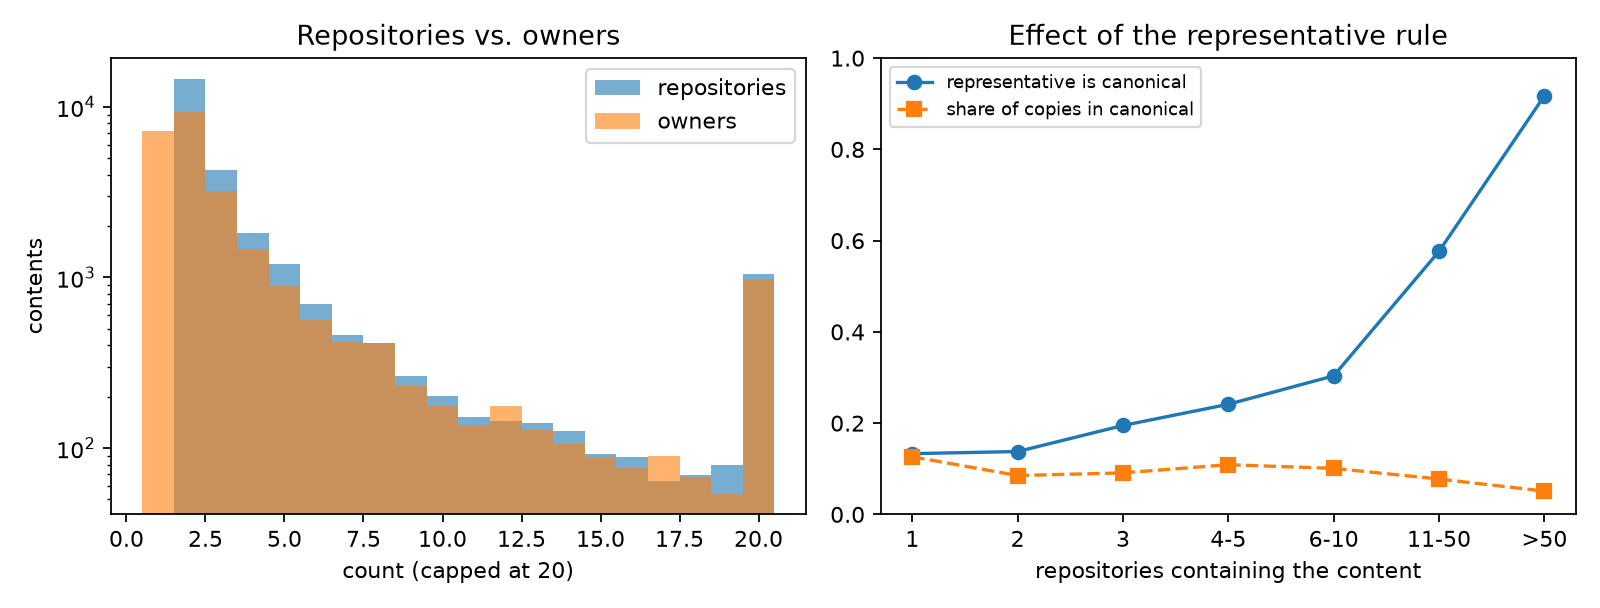
\includegraphics[width=0.82\linewidth]{figures/report_eda_owner_and_selection.png}
\caption{Distributions of repositories and owners (left) and effect of the representative rule (right)}
\label{fig:report-1}
\end{figure}

In the first version of the study, with \texttt{repository\_count} as
target and repository attributes, this inflated the result. With the
Random Forest and the full development set, the repository attributes
gave an RMSLE of 0.575; without \texttt{history\_fetched} and
\texttt{commit\_count}, 0.604 (difference of +0.029, 95\% CI {[}0.018;
0.040{]}), against 0.623 for the mean-of-\texttt{log1p} baseline. The
location of the representative alone (three categories) gave 0.584, and
the history alone 0.594. The ``repository'' view was, to a large extent,
a proxy for location.

\subsection{Main protocol}\label{main-protocol}

With the shortcuts out, 17,733 contents (cap of 50 per owner) and
owner-grouped validation, the results of the Random Forest (RF) and of
the linear models are:

\begin{longtable}[]{@{}
  >{\raggedright\arraybackslash}p{(\linewidth - 8\tabcolsep) * \real{0.1579}}
  >{\raggedleft\arraybackslash}p{(\linewidth - 8\tabcolsep) * \real{0.2105}}
  >{\raggedleft\arraybackslash}p{(\linewidth - 8\tabcolsep) * \real{0.2105}}
  >{\raggedleft\arraybackslash}p{(\linewidth - 8\tabcolsep) * \real{0.2105}}
  >{\raggedleft\arraybackslash}p{(\linewidth - 8\tabcolsep) * \real{0.2105}}@{}}
\caption{Performance by view (mean ± standard deviation over 9
owner-grouped folds).}\tabularnewline
\toprule\noalign{}
\begin{minipage}[b]{\linewidth}\raggedright
View
\end{minipage} & \begin{minipage}[b]{\linewidth}\raggedleft
RF AUC
\end{minipage} & \begin{minipage}[b]{\linewidth}\raggedleft
logistic AUC
\end{minipage} & \begin{minipage}[b]{\linewidth}\raggedleft
RF RMSLE
\end{minipage} & \begin{minipage}[b]{\linewidth}\raggedleft
Ridge RMSLE
\end{minipage} \\
\midrule\noalign{}
\endfirsthead
\toprule\noalign{}
\begin{minipage}[b]{\linewidth}\raggedright
View
\end{minipage} & \begin{minipage}[b]{\linewidth}\raggedleft
RF AUC
\end{minipage} & \begin{minipage}[b]{\linewidth}\raggedleft
logistic AUC
\end{minipage} & \begin{minipage}[b]{\linewidth}\raggedleft
RF RMSLE
\end{minipage} & \begin{minipage}[b]{\linewidth}\raggedleft
Ridge RMSLE
\end{minipage} \\
\midrule\noalign{}
\endhead
\bottomrule\noalign{}
\endlastfoot
skill & 0.660 ± 0.022 & 0.614 & 0.698 ± 0.007 & 0.713 \\
repository & 0.650 ± 0.019 & 0.655 & 0.707 ± 0.011 & 0.702 \\
repository + catalog & 0.666 ± 0.009 & 0.662 & 0.696 ± 0.010 & 0.699 \\
path + catalog & 0.579 ± 0.019 & 0.576 & 0.718 ± 0.018 & 0.714 \\
\textbf{clean (full)} & \textbf{0.716 ± 0.024} & 0.680 & \textbf{0.679 ±
0.011} & 0.694 \\
clean + shortcuts & 0.717 ± 0.022 & 0.682 & 0.637 ± 0.015 & 0.664 \\
shortcuts only & 0.500 ± 0.015 & 0.510 & 0.688 ± 0.010 & 0.693 \\
\emph{baseline} & 0.500 & 0.500 & 0.720 (mean), 0.780 (median) & \\
\end{longtable}

All pre-specified hypotheses are rejected after Holm correction:

\begin{longtable}[]{@{}
  >{\raggedright\arraybackslash}p{(\linewidth - 8\tabcolsep) * \real{0.1875}}
  >{\raggedright\arraybackslash}p{(\linewidth - 8\tabcolsep) * \real{0.1875}}
  >{\raggedright\arraybackslash}p{(\linewidth - 8\tabcolsep) * \real{0.1875}}
  >{\raggedright\arraybackslash}p{(\linewidth - 8\tabcolsep) * \real{0.1875}}
  >{\raggedleft\arraybackslash}p{(\linewidth - 8\tabcolsep) * \real{0.2500}}@{}}
\caption{Pre-specified hypotheses on development (exploratory until the
confirmation of Section 4.7).}\tabularnewline
\toprule\noalign{}
\begin{minipage}[b]{\linewidth}\raggedright
\end{minipage} & \begin{minipage}[b]{\linewidth}\raggedright
Comparison
\end{minipage} & \begin{minipage}[b]{\linewidth}\raggedright
Result
\end{minipage} & \begin{minipage}[b]{\linewidth}\raggedright
95\% CI of the difference
\end{minipage} & \begin{minipage}[b]{\linewidth}\raggedleft
p (Holm)
\end{minipage} \\
\midrule\noalign{}
\endfirsthead
\toprule\noalign{}
\begin{minipage}[b]{\linewidth}\raggedright
\end{minipage} & \begin{minipage}[b]{\linewidth}\raggedright
Comparison
\end{minipage} & \begin{minipage}[b]{\linewidth}\raggedright
Result
\end{minipage} & \begin{minipage}[b]{\linewidth}\raggedright
95\% CI of the difference
\end{minipage} & \begin{minipage}[b]{\linewidth}\raggedleft
p (Holm)
\end{minipage} \\
\midrule\noalign{}
\endhead
\bottomrule\noalign{}
\endlastfoot
H1 & clean RF AUC against 0.5 & 0.716 & +0.216 {[}0.173; 0.259{]} &
\textless{} 0.001 \\
H2 & clean RF RMSLE against the mean & 0.679 vs 0.720 & −0.041
{[}−0.049; −0.033{]} & \textless{} 0.001 \\
H3a & clean against repository+catalog (AUC) & 0.716 vs 0.666 & +0.050
{[}0.017; 0.083{]} & 0.008 \\
H3b & clean against skill (AUC) & 0.716 vs 0.660 & +0.056 {[}0.040;
0.072{]} & \textless{} 0.001 \\
H4 & clean+shortcuts against clean (RMSLE) & 0.637 vs 0.679 & −0.042
{[}−0.055; −0.029{]} & \textless{} 0.001 \\
\end{longtable}

There is a real but modest signal: an AUC of 0.72 and a 6\% reduction in
RMSLE. Skill and repository contribute \textbf{complementarily}: each
block alone sits at AUC 0.65--0.67, and the combination at 0.72 (H3a and
H3b). The shortcuts add to the regression (H4) but, alone, do not
predict cross-owner reuse (AUC 0.50): the regression gain comes from
their correlation with the number of copies, not from cross-owner reuse.
The path, in isolation, barely predicts.

\subsection{Robustness}\label{robustness}

\textbf{Per-owner cap.} The performance of the clean RF changes little
in RMSLE, but a lot in AUC, depending on how concentrated owners are
treated:

\begin{longtable}[]{@{}
  >{\raggedright\arraybackslash}p{(\linewidth - 8\tabcolsep) * \real{0.1579}}
  >{\raggedleft\arraybackslash}p{(\linewidth - 8\tabcolsep) * \real{0.2105}}
  >{\raggedleft\arraybackslash}p{(\linewidth - 8\tabcolsep) * \real{0.2105}}
  >{\raggedleft\arraybackslash}p{(\linewidth - 8\tabcolsep) * \real{0.2105}}
  >{\raggedleft\arraybackslash}p{(\linewidth - 8\tabcolsep) * \real{0.2105}}@{}}
\caption{Sensitivity to the treatment of concentrated owners (RF,
baseline = mean of \texttt{log1p}).}\tabularnewline
\toprule\noalign{}
\begin{minipage}[b]{\linewidth}\raggedright
Treatment
\end{minipage} & \begin{minipage}[b]{\linewidth}\raggedleft
contents
\end{minipage} & \begin{minipage}[b]{\linewidth}\raggedleft
clean RF AUC
\end{minipage} & \begin{minipage}[b]{\linewidth}\raggedleft
RMSLE gain (clean)
\end{minipage} & \begin{minipage}[b]{\linewidth}\raggedleft
gain (shortcuts only)
\end{minipage} \\
\midrule\noalign{}
\endfirsthead
\toprule\noalign{}
\begin{minipage}[b]{\linewidth}\raggedright
Treatment
\end{minipage} & \begin{minipage}[b]{\linewidth}\raggedleft
contents
\end{minipage} & \begin{minipage}[b]{\linewidth}\raggedleft
clean RF AUC
\end{minipage} & \begin{minipage}[b]{\linewidth}\raggedleft
RMSLE gain (clean)
\end{minipage} & \begin{minipage}[b]{\linewidth}\raggedleft
gain (shortcuts only)
\end{minipage} \\
\midrule\noalign{}
\endhead
\bottomrule\noalign{}
\endlastfoot
no limit & 25,918 & 0.747 ± 0.140 & 0.039 & 0.040 \\
exclude owners with more than 1000 & 21,615 & 0.615 ± 0.036 & 0.036 &
0.040 \\
exclude owners with more than 500 & 19,567 & 0.708 ± 0.037 & 0.030 &
0.041 \\
exclude owners with more than 200 & 18,443 & 0.732 ± 0.035 & 0.037 &
0.040 \\
\textbf{50 per owner} & 17,733 & 0.716 ± 0.024 & 0.041 & 0.031 \\
\end{longtable}

The RMSLE is stable (gain of 0.03--0.04), but the AUC oscillates from
0.615 to 0.747: a few owners with 500 to 1000 contents lower the AUC by
0.1, and with no limit a single fold concentrates one owner and the
standard deviation reaches 0.14. Performance therefore depends on the
composition of a dozen accounts. The cap of 50 stabilizes the estimates,
but it is a data-dependent choice.

\textbf{Other checks.} (i) Fixing the location class and training within
each one (owners with more than 500 contents excluded), the clean RF
still beats the baseline: \texttt{canonical} (5,439 contents) RMSLE
−0.141 and AUC 0.714; \texttt{skills-dir} (10,721) −0.013 and 0.672;
\texttt{other} (3,810) −0.011 and 0.828. The signal is not only
location. (ii) With \texttt{repository\_count} as target, the gain of
the clean RF is the same (−0.031 versus −0.030). (iii) Only 18.8\% of
validation rows have a \texttt{name} seen in training; on the subset
without overlap the gain persists (RMSLE −0.039 versus −0.041 on all;
AUC 0.726 versus 0.716), which indicates that variants of the same
\texttt{name} do not explain the result. (iv) Repository-grouped
validation, instead of owner-grouped, did not produce larger estimates
(RMSLE 0.657 versus 0.655; AUC 0.735 versus 0.747, with the standard
deviation of 0.14 of the no-limit case).

\subsection{Interpretation}\label{interpretation}

\begin{figure}[!htbp]
\centering
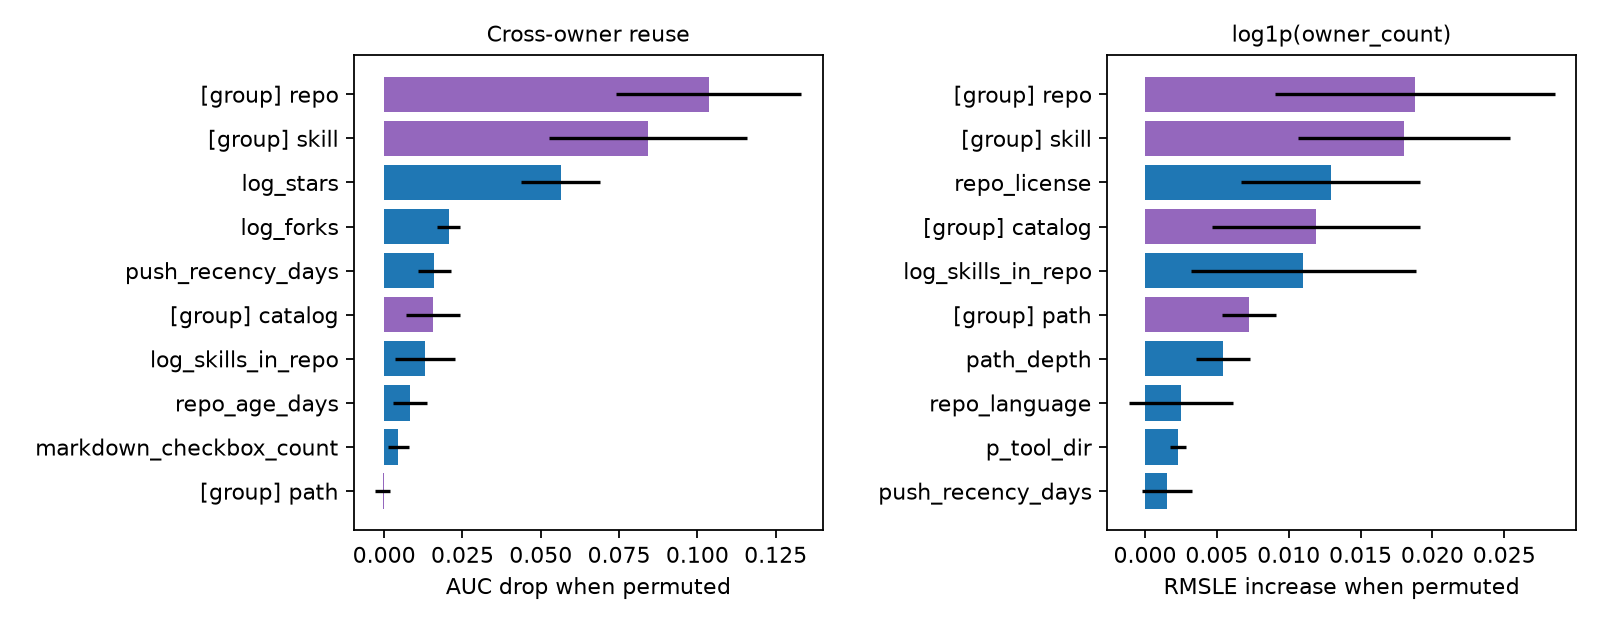
\includegraphics[width=0.82\linewidth]{figures/report_permutation_importance.png}
\caption{Permutation importance of the clean RF (owner-grouped folds; owners with more than 500 contents excluded)}
\label{fig:report-2}
\end{figure}

For cross-owner reuse, the repository block weighs more (AUC drop of
0.104 when permuted) than skill (0.084), catalog (0.016) and path (≈ 0).
Among columns, \texttt{log\_stars} dominates (0.056), followed by
\texttt{log\_forks} (0.021) and push recency (0.016): skills in more
visible repositories are copied more by other owners. In regression,
repository (0.019) and skill (0.018) weigh similarly, and the largest
column is the license (0.013), followed by catalog size (0.011) and path
depth (0.005). We could not identify why the license weighs so much; it
may be an indicator of repositories that clone catalogs. Uncertainties
are large (6 folds), and the correlation among attributes limits the
individual reading.

\subsection{Model selection and
tuning}\label{model-selection-and-tuning}

\begin{longtable}[]{@{}lrrrr@{}}
\caption{Nested validation (mean of 6 outer owner-grouped folds; 6
candidates per search).}\tabularnewline
\toprule\noalign{}
Family & AUC default & AUC searched & RMSLE default & RMSLE searched \\
\midrule\noalign{}
\endfirsthead
\toprule\noalign{}
Family & AUC default & AUC searched & RMSLE default & RMSLE searched \\
\midrule\noalign{}
\endhead
\bottomrule\noalign{}
\endlastfoot
linear & 0.678 & 0.689 & 0.692 & 0.690 \\
KNN & 0.667 & 0.690 & 0.703 & 0.686 \\
tree & 0.614 & 0.634 & 0.807 & 0.699 \\
Random Forest & \textbf{0.716} & 0.701 & 0.679 & 0.675 \\
Gradient Boosting & 0.691 & 0.704 & 0.690 & 0.671 \\
HistGradientBoosting & 0.693 & 0.682 & \textbf{0.670} & 0.688 \\
\emph{baseline} & 0.500 & & 0.720 & \\
\end{longtable}

By the pre-specified rule, we froze the default RF (classification) and
the default HistGradientBoosting (regression). \textbf{The families
tie:} the RF against the runner-up (searched Gradient Boosting) has an
AUC difference of 0.012 (95\% CI {[}−0.003; 0.026{]}), and in regression
the HistGB against the searched Gradient Boosting has −0.001 {[}−0.027;
0.024{]}. Only the decision tree (and, with less evidence, the default
KNN) falls behind, and in classification even these differences do not
survive Holm correction (p between 0.06 and 0.13). The hyperparameter
search did not beat the default configuration (RF classification:
default 0.716 versus searched 0.701).

\subsection{Confirmation on the
holdout}\label{confirmation-on-the-holdout}

The frozen models were evaluated once on 25,011 contents from 10,484
owners disjoint from development.

\begin{longtable}[]{@{}
  >{\raggedright\arraybackslash}p{(\linewidth - 8\tabcolsep) * \real{0.1765}}
  >{\raggedright\arraybackslash}p{(\linewidth - 8\tabcolsep) * \real{0.1765}}
  >{\raggedleft\arraybackslash}p{(\linewidth - 8\tabcolsep) * \real{0.2353}}
  >{\raggedleft\arraybackslash}p{(\linewidth - 8\tabcolsep) * \real{0.2353}}
  >{\raggedright\arraybackslash}p{(\linewidth - 8\tabcolsep) * \real{0.1765}}@{}}
\caption{Single evaluation on the holdout.}\tabularnewline
\toprule\noalign{}
\begin{minipage}[b]{\linewidth}\raggedright
Task
\end{minipage} & \begin{minipage}[b]{\linewidth}\raggedright
Model
\end{minipage} & \begin{minipage}[b]{\linewidth}\raggedleft
Result
\end{minipage} & \begin{minipage}[b]{\linewidth}\raggedleft
Baseline
\end{minipage} & \begin{minipage}[b]{\linewidth}\raggedright
95\% CI (owner bootstrap)
\end{minipage} \\
\midrule\noalign{}
\endfirsthead
\toprule\noalign{}
\begin{minipage}[b]{\linewidth}\raggedright
Task
\end{minipage} & \begin{minipage}[b]{\linewidth}\raggedright
Model
\end{minipage} & \begin{minipage}[b]{\linewidth}\raggedleft
Result
\end{minipage} & \begin{minipage}[b]{\linewidth}\raggedleft
Baseline
\end{minipage} & \begin{minipage}[b]{\linewidth}\raggedright
95\% CI (owner bootstrap)
\end{minipage} \\
\midrule\noalign{}
\endhead
\bottomrule\noalign{}
\endlastfoot
\texttt{cross\_owner} & Random Forest & AUC \textbf{0.731}; PR AUC
0.913; Brier 0.140; log-loss 0.444 & 0.5; 0.808; 0.155; 0.490 & AUC
{[}0.716; 0.745{]}; PR AUC {[}0.905; 0.921{]} \\
\texttt{log1p(owner\_count)} & HistGradientBoosting & RMSLE
\textbf{0.625}; Spearman 0.330 & 0.664 (mean of \texttt{log1p}) &
difference −0.038 {[}−0.044; −0.032{]} \\
\end{longtable}

\begin{figure}[!htbp]
\centering
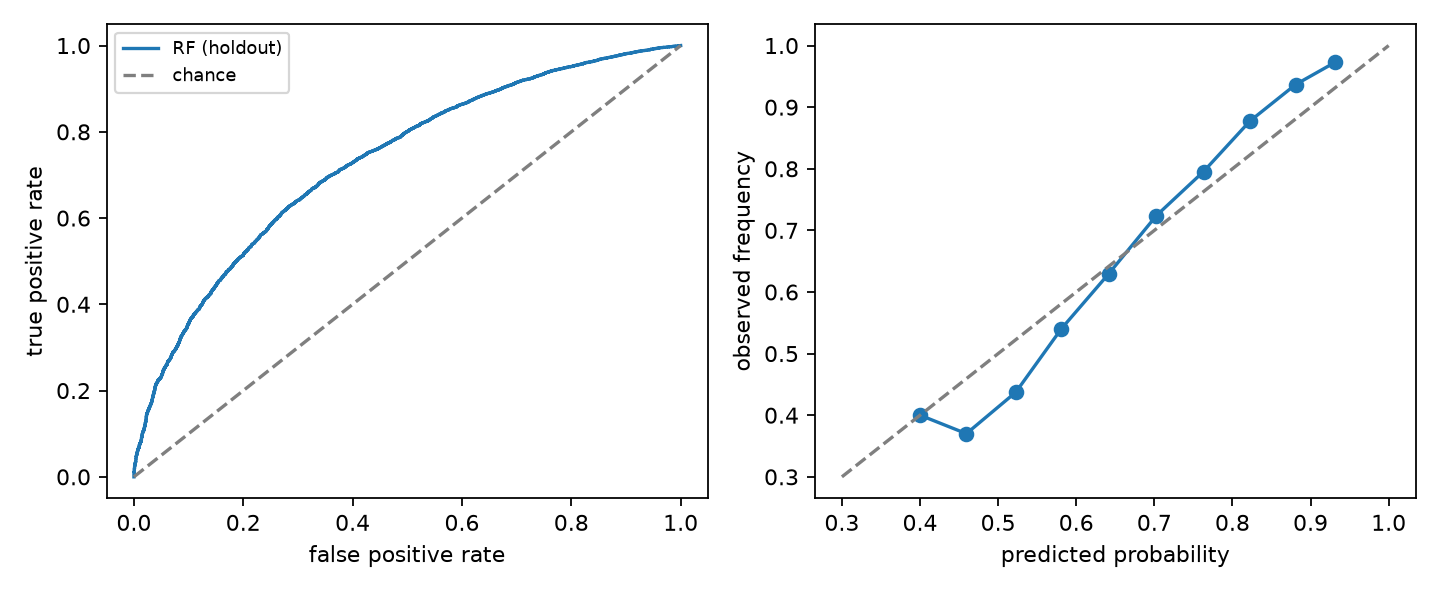
\includegraphics[width=0.82\linewidth]{figures/report_holdout_roc_calibration.png}
\caption{ROC curve and calibration of the RF on the holdout}
\label{fig:report-3}
\end{figure}

The success criteria were met: the lower AUC bound is above 0.5 and the
upper bound of the RMSLE difference is below zero. The holdout AUC
(0.731) is consistent with the nested estimate on development (0.716).
The holdout has a different composition (36\% \texttt{canonical} skills
versus 21\% in development, and 9\% \texttt{other} versus 21\%), since
concentrated owners are left out by construction. H3 and H4 were not
re-evaluated on the holdout and remain exploratory.
